% PettingZoo-Bibliothek

Als Grundlage für die Messumgebung dient die Open Source Python-Bibliothek PettingZoo, die zum Entwickeln und Testen von MARL-Systemen konzipiert wurde. Sie stellt eine einheitliche Schnittstelle zu Umgebungen bereit, in der Agenten miteinander interagieren können.

Die Umgebungen definieren den Rahmen, in dem die Agenten miteinander interagieren. Sie weisen ein bestimmtes Verhalten auf und definieren unter anderem, unter welchen Bedingungen welche Aktionen möglich sind, Belohnungen verteilt werden und in welcher Form die Agenten Informationen über den Zustand der Umgebung erhalten. Es existieren eine Reihe von vorgefertigten Umgebungen, darunter welche, die kooperative Probleme zum Benchmarking von MARL-Systemen oder auch rundenbasierte Spiele wie Vier Gewinnt abbilden.

Die durch PettingZoo bereitgestellte Schnittstelle ermöglicht es, aus Sicht eines Agenten den aktuellen Zustand der Umgebung zu beobachten, die im aktuellen Zustand möglichen Aktionen und erhaltenen Belohnungen zu ermitteln und eine Aktion auszuwählen, die in der Umgebung durchgeführt werden soll.

Für alle Agenten der Umgebung kann benutzerdefinierte Logik eingebunden werden, die bestimmt, wie sie ihre Aktionen wählen. Vorgesehen sind dabei RL-Modelle, es können jedoch auch symbolische Algorithmen eingesetzt werden, darunter auch welche, die ihre Entscheidungen rein zufällig oder unter Einbezug von menschlichen Eingaben treffen \cite{Farama.2025}.

% Implementierung der Messumgebung

Die Implementierung der Messumgebung baut auf der offiziellen Implementierung der Vier-Gewinnt-Umgebung von PettingZoo auf. Die Messumgebung tut dabei nichts anderes, als wiederholt zwei Agenten mit bestimmten Lösungsansätzen das Spiel spielen zu lassen und dabei die Gewinnraten und Spieldauer zu messen. Die Open-Source-Eigenschaft ermöglicht es, den Quellcode zu modifizieren. Davon wird im weiteren Verlauf der Arbeit Gebrauch gemacht, unter anderem, um die verschiedenen Szenarien zur Untersuchung von Robustheit abzubilden.

Im Zuge der Realisierung der Messumgebung ist aufgefallen, dass wenn zwei Agenten (Spieler 0 und Spieler 1) alle Aktionen im Spiel mit derselben Wahrscheinlichkeit rein zufällig wählen, nach 1000 Spielen Spieler 0 mit 55,20 \% gegenüber Spieler 1 mit 44,30 \% eine wesentlich höhere Gewinnrate erzielt.

\begin{figure}[ht!]%[!tbp]
	\begin{subfigure}[b]{0.48\textwidth}
		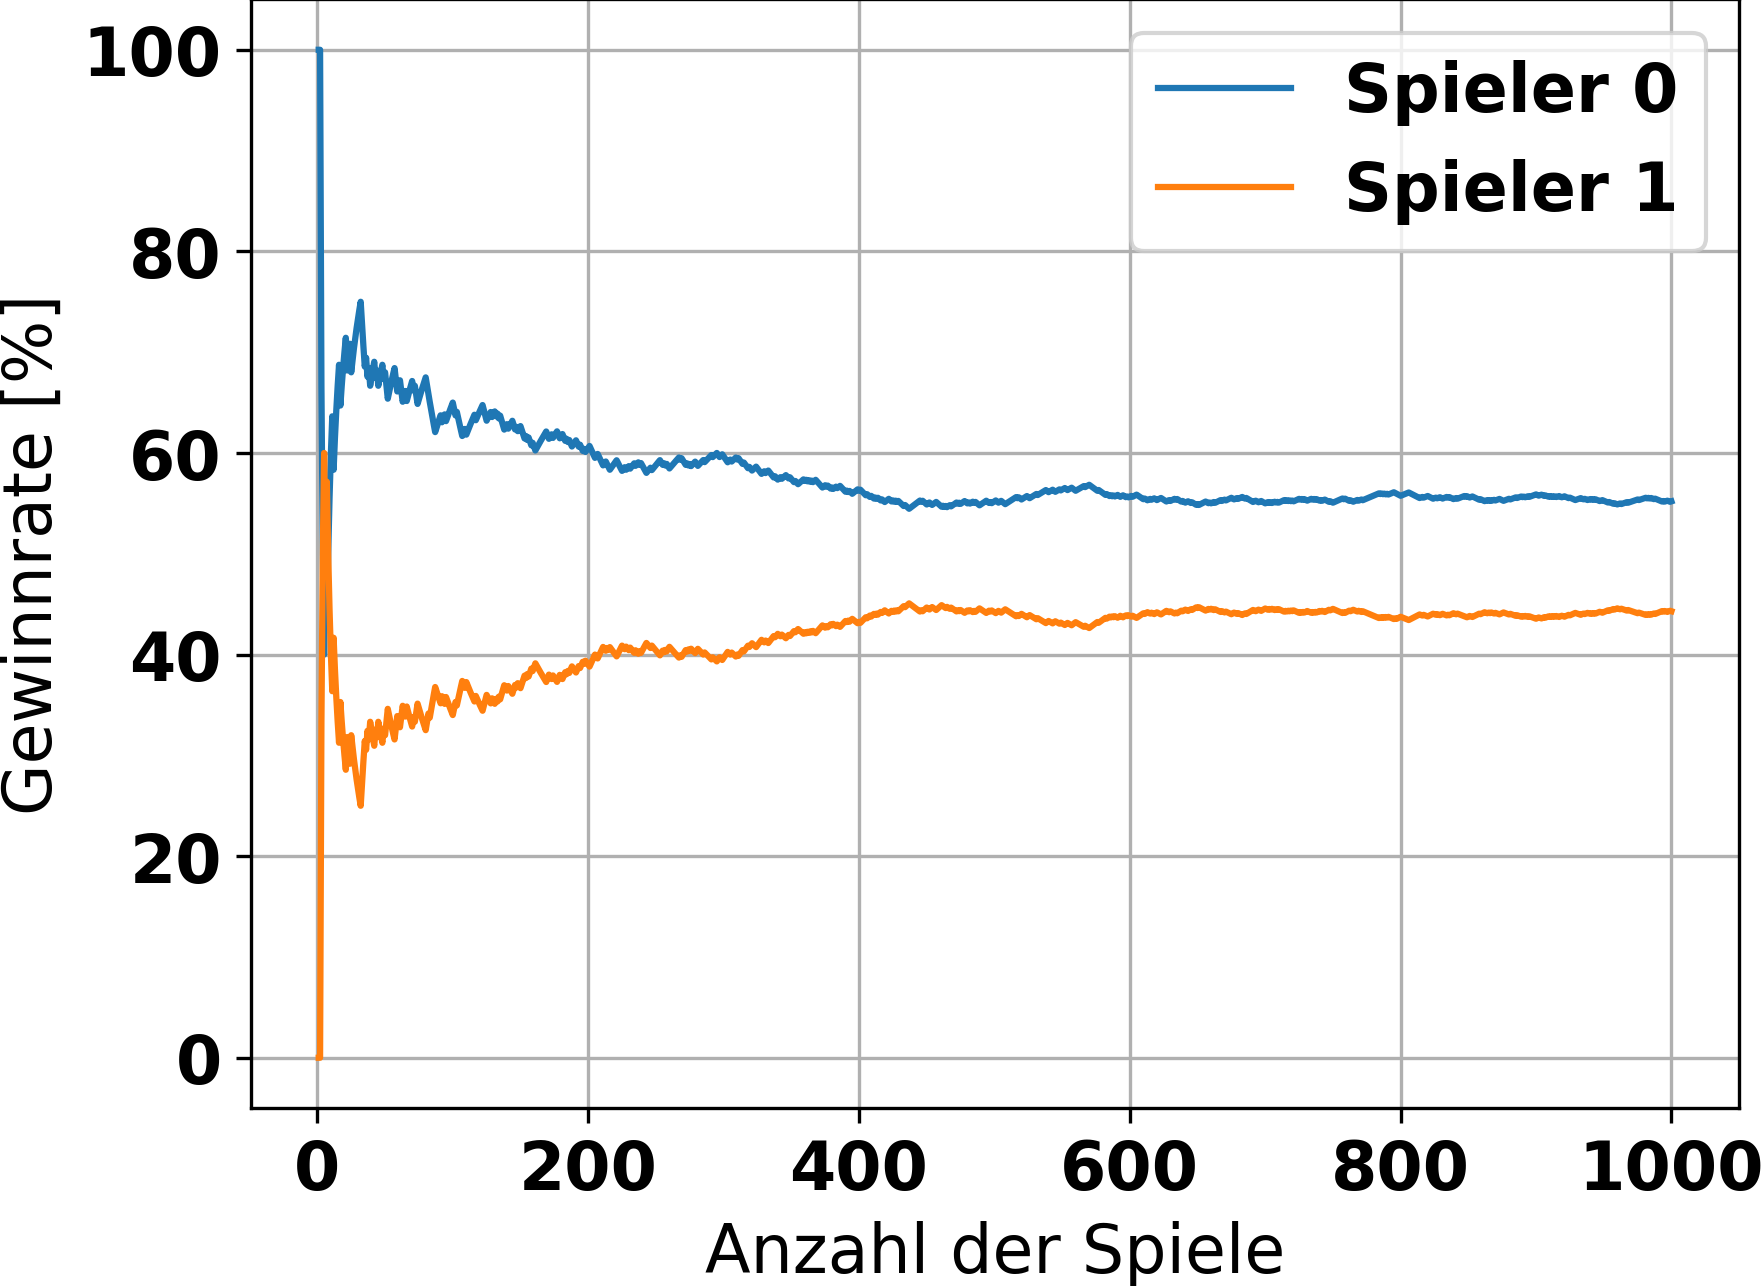
\includegraphics[width=\textwidth]{Bilder/constant_player_order_graph_win_rates.png}
		\caption{Gewinnrate.}
		\label{fig:f1}
	\end{subfigure}
	\hfill
	\begin{subfigure}[b]{0.48\textwidth}
		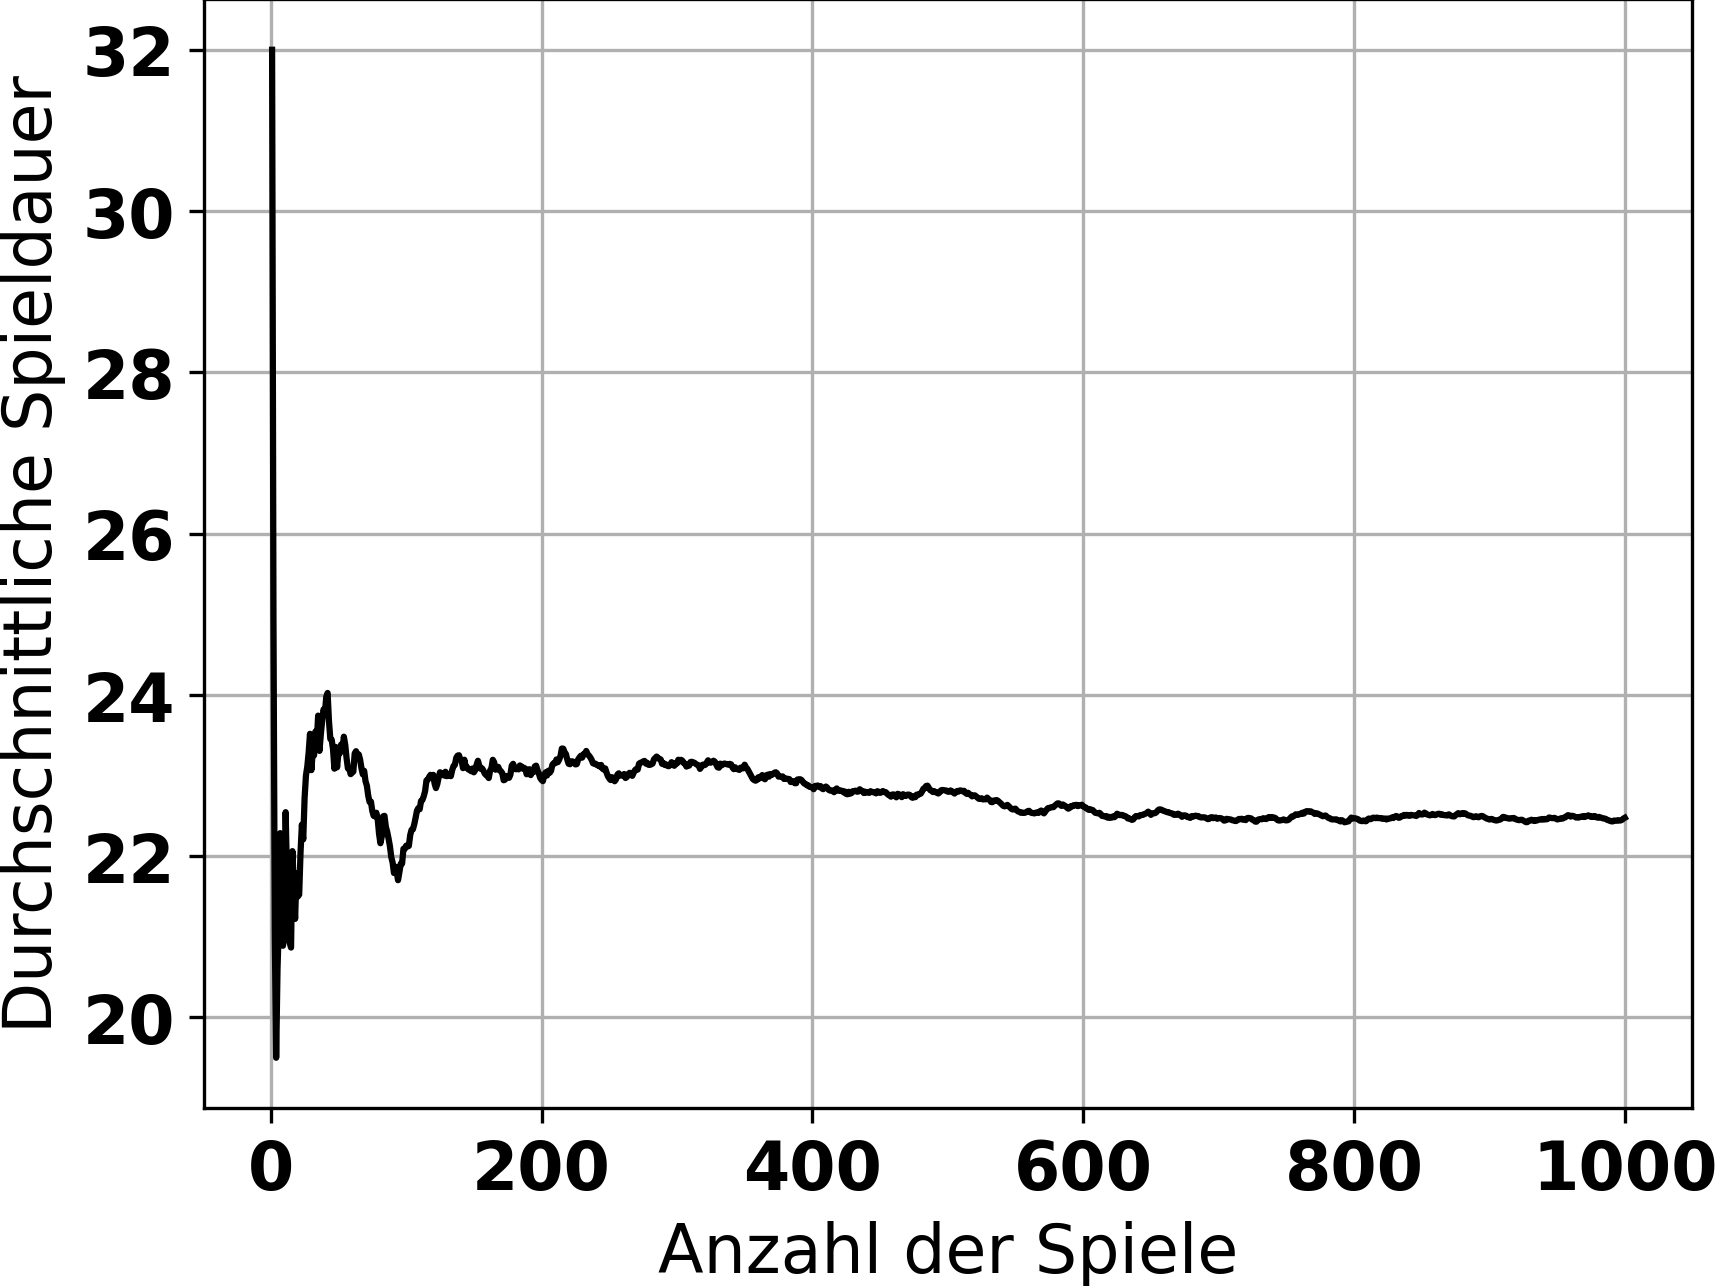
\includegraphics[width=\textwidth]{Bilder/constant_player_order_graph_game_length.png}
		\caption{Durchschnittliche Spieldauer.}
		\label{fig:f2}
	\end{subfigure}
	\caption{Gewinnrate und durchschnittliche Spieldauer bei konstanter Spielerreihenfolge.}
\end{figure}

Das lässt sich dadurch erklären, dass die Vier-Gewinnt-Umgebung so implementiert ist, dass Spieler 0 immer der Spieler ist, der den ersten Stein setzen darf. Er ist damit seinem Gegenspieler immer einen Spielzug voraus, was die Wahrscheinlichkeit erhöht, als erstes Vier Steine in eine Reihe zu bekommen. An dieser Stelle sei nochmals zu erwähnen, dass bei Vier Gewinnt der erste Spieler bei optimaler Spielweise stets gewinnen kann. Um ausgeglichene Messungen zu gewährleisten, muss daher sichergestellt werden, dass sich im Rahmen der Messungen die beiden Spieler mit dem ersten Zug abwechseln.

Die Vier-Gewinnt-Umgebung von PettingZoo wurde daher erweitert, um einen Parameter entgegenzunehmen und zu verarbeiten, der bestimmt, welcher Spieler anfangen soll. Die Messumgebung wechselt den Wert des Parameters nach jedem Spiel durch. Nach dieser Änderung weisen die Spiele wesentlich ausgeglichenere Ergebnisse auf. Spieler 0 gewinnt 50,30 \% und Spieler 1 49,50 \% der Spiele. Die durchschnittliche Spieldauer bleibt dabei mit 22,48 Zügen vor der Änderung gegenüber 22,26 Zügen nach der Änderung nahezu unverändert.

\begin{figure}[ht!]%[!tbp]
	\begin{subfigure}[b]{0.48\textwidth}
		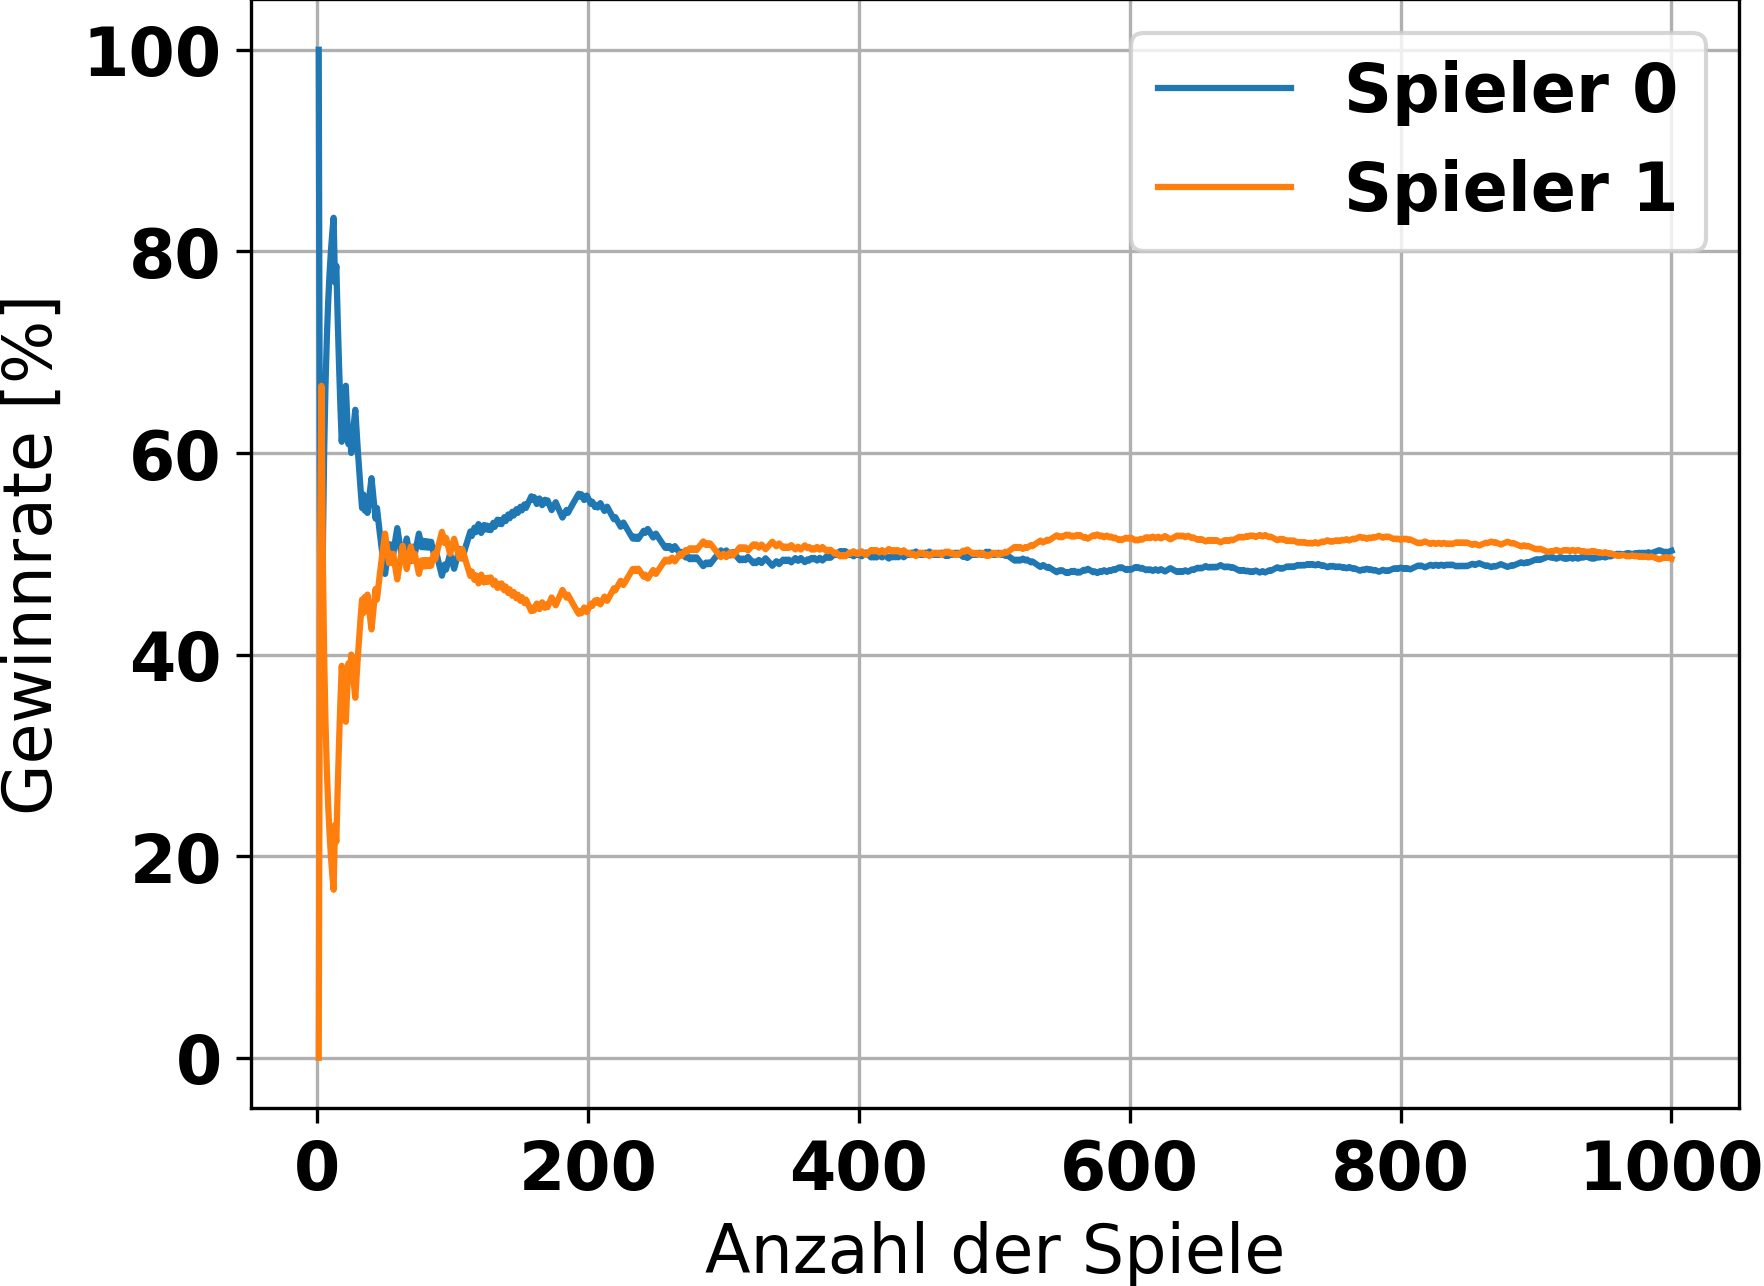
\includegraphics[width=\textwidth]{Bilder/alternating_player_order_graph_win_rates.png}
		\caption{Gewinnrate.}
		\label{fig:f3}
	\end{subfigure}
	\hfill
	\begin{subfigure}[b]{0.48\textwidth}
		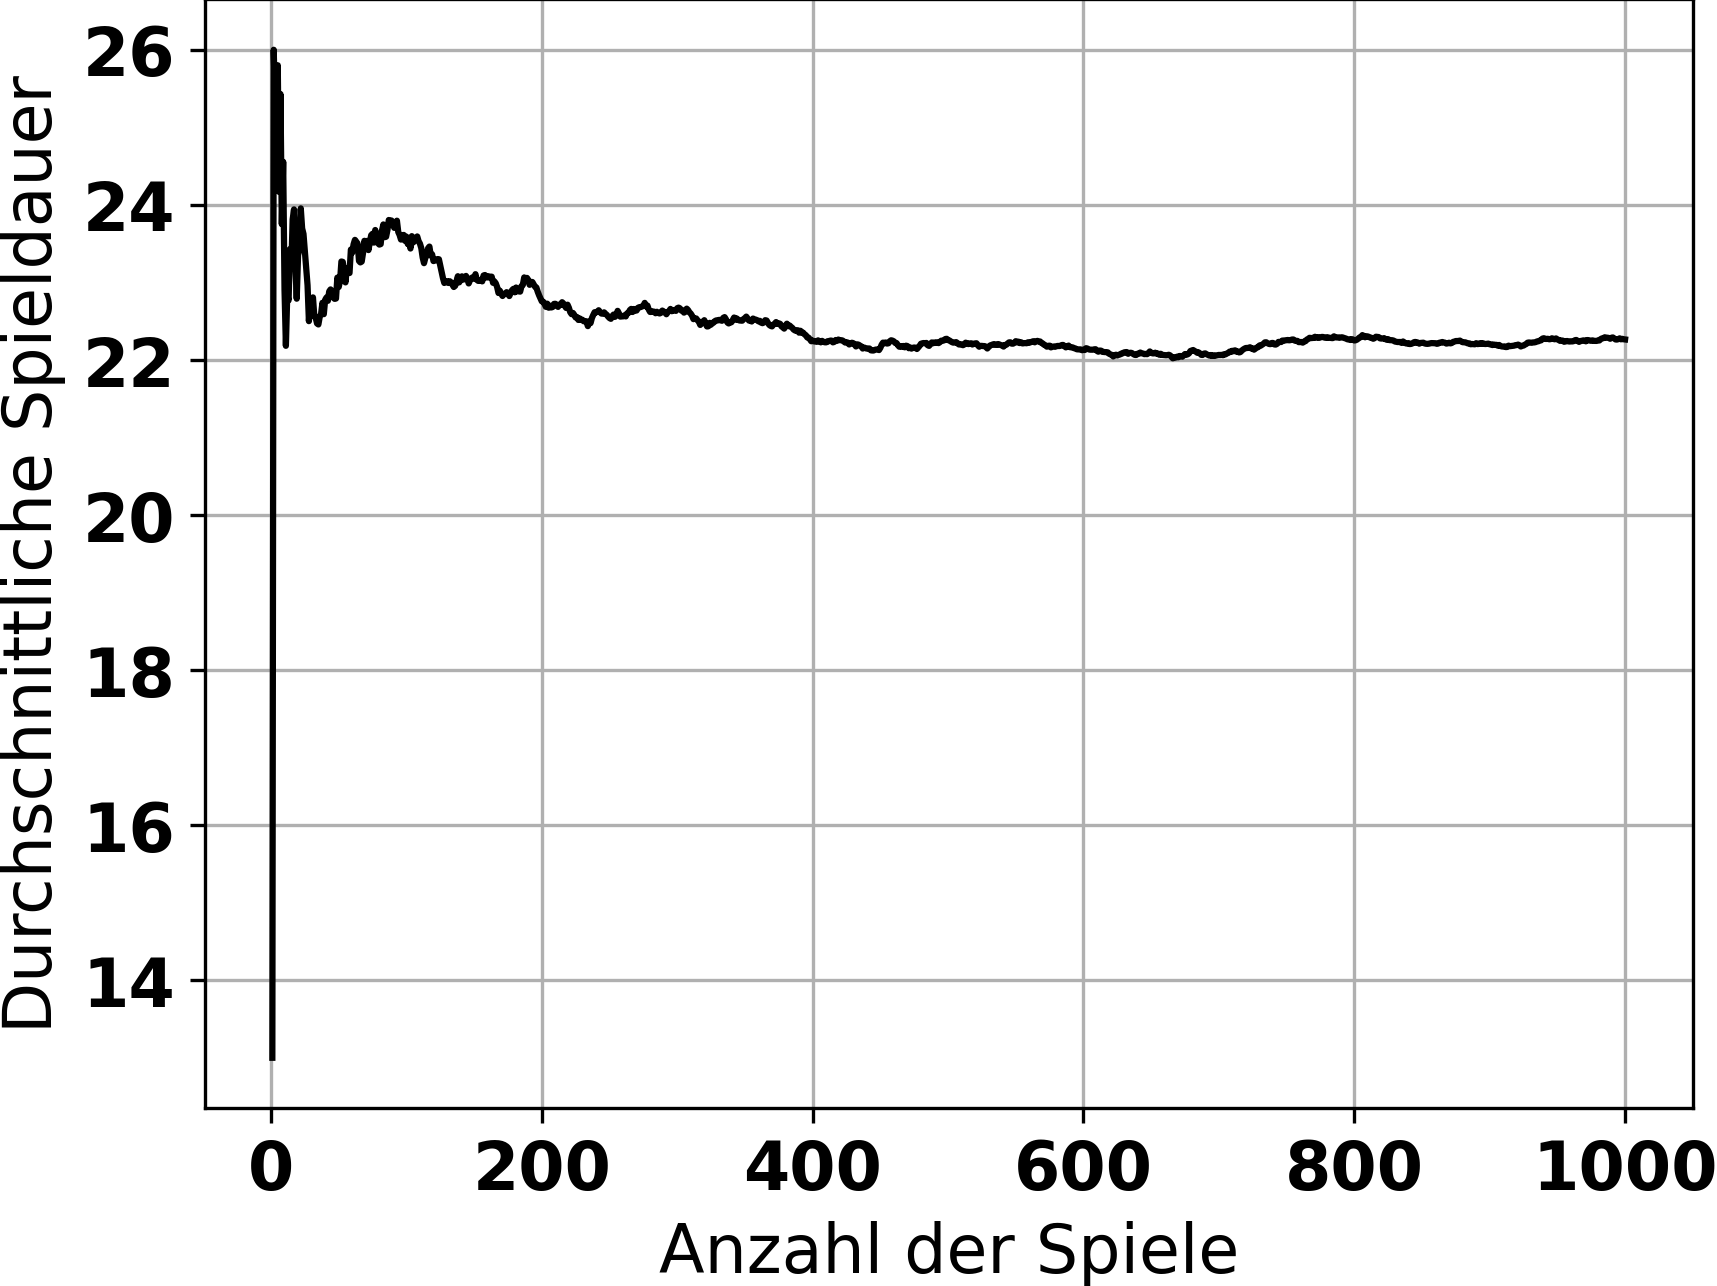
\includegraphics[width=\textwidth]{Bilder/alternating_player_order_graph_game_length.png}
		\caption{Durchschnittliche Spieldauer.}
		\label{fig:f4}
	\end{subfigure}
	\caption{Gewinnrate und durchschnittliche Spieldauer bei abwechselnder Spielerreihenfolge.}
\end{figure}

% Es kommen Reinforcement Learning Modelle zum Einsatz, die aus RL-Bibliotheken wie CleanRL oder Stable-Baselines bereitgestellt werden. Falls vorhanden, wird auf fertig implementierte Algorithmen zurückgegriffen.

\newpage